\documentclass{article}

\usepackage{graphicx}
\usepackage{tikz}
\usepackage{tikzsymbols}
\usetikzlibrary{calc,patterns,shapes.geometric}
\pagestyle{empty}
\usepackage[margin=0pt]{geometry}
\geometry{papersize={14in,12in}}

\def\centerarc[#1](#2)(#3:#4:#5){\draw[#1] ($(#2)+({#5*cos(#3)},{#5*sin(#3)})$) arc (#3:#4:#5);}

\begin{document}
	\begin{figure}
		\centering
		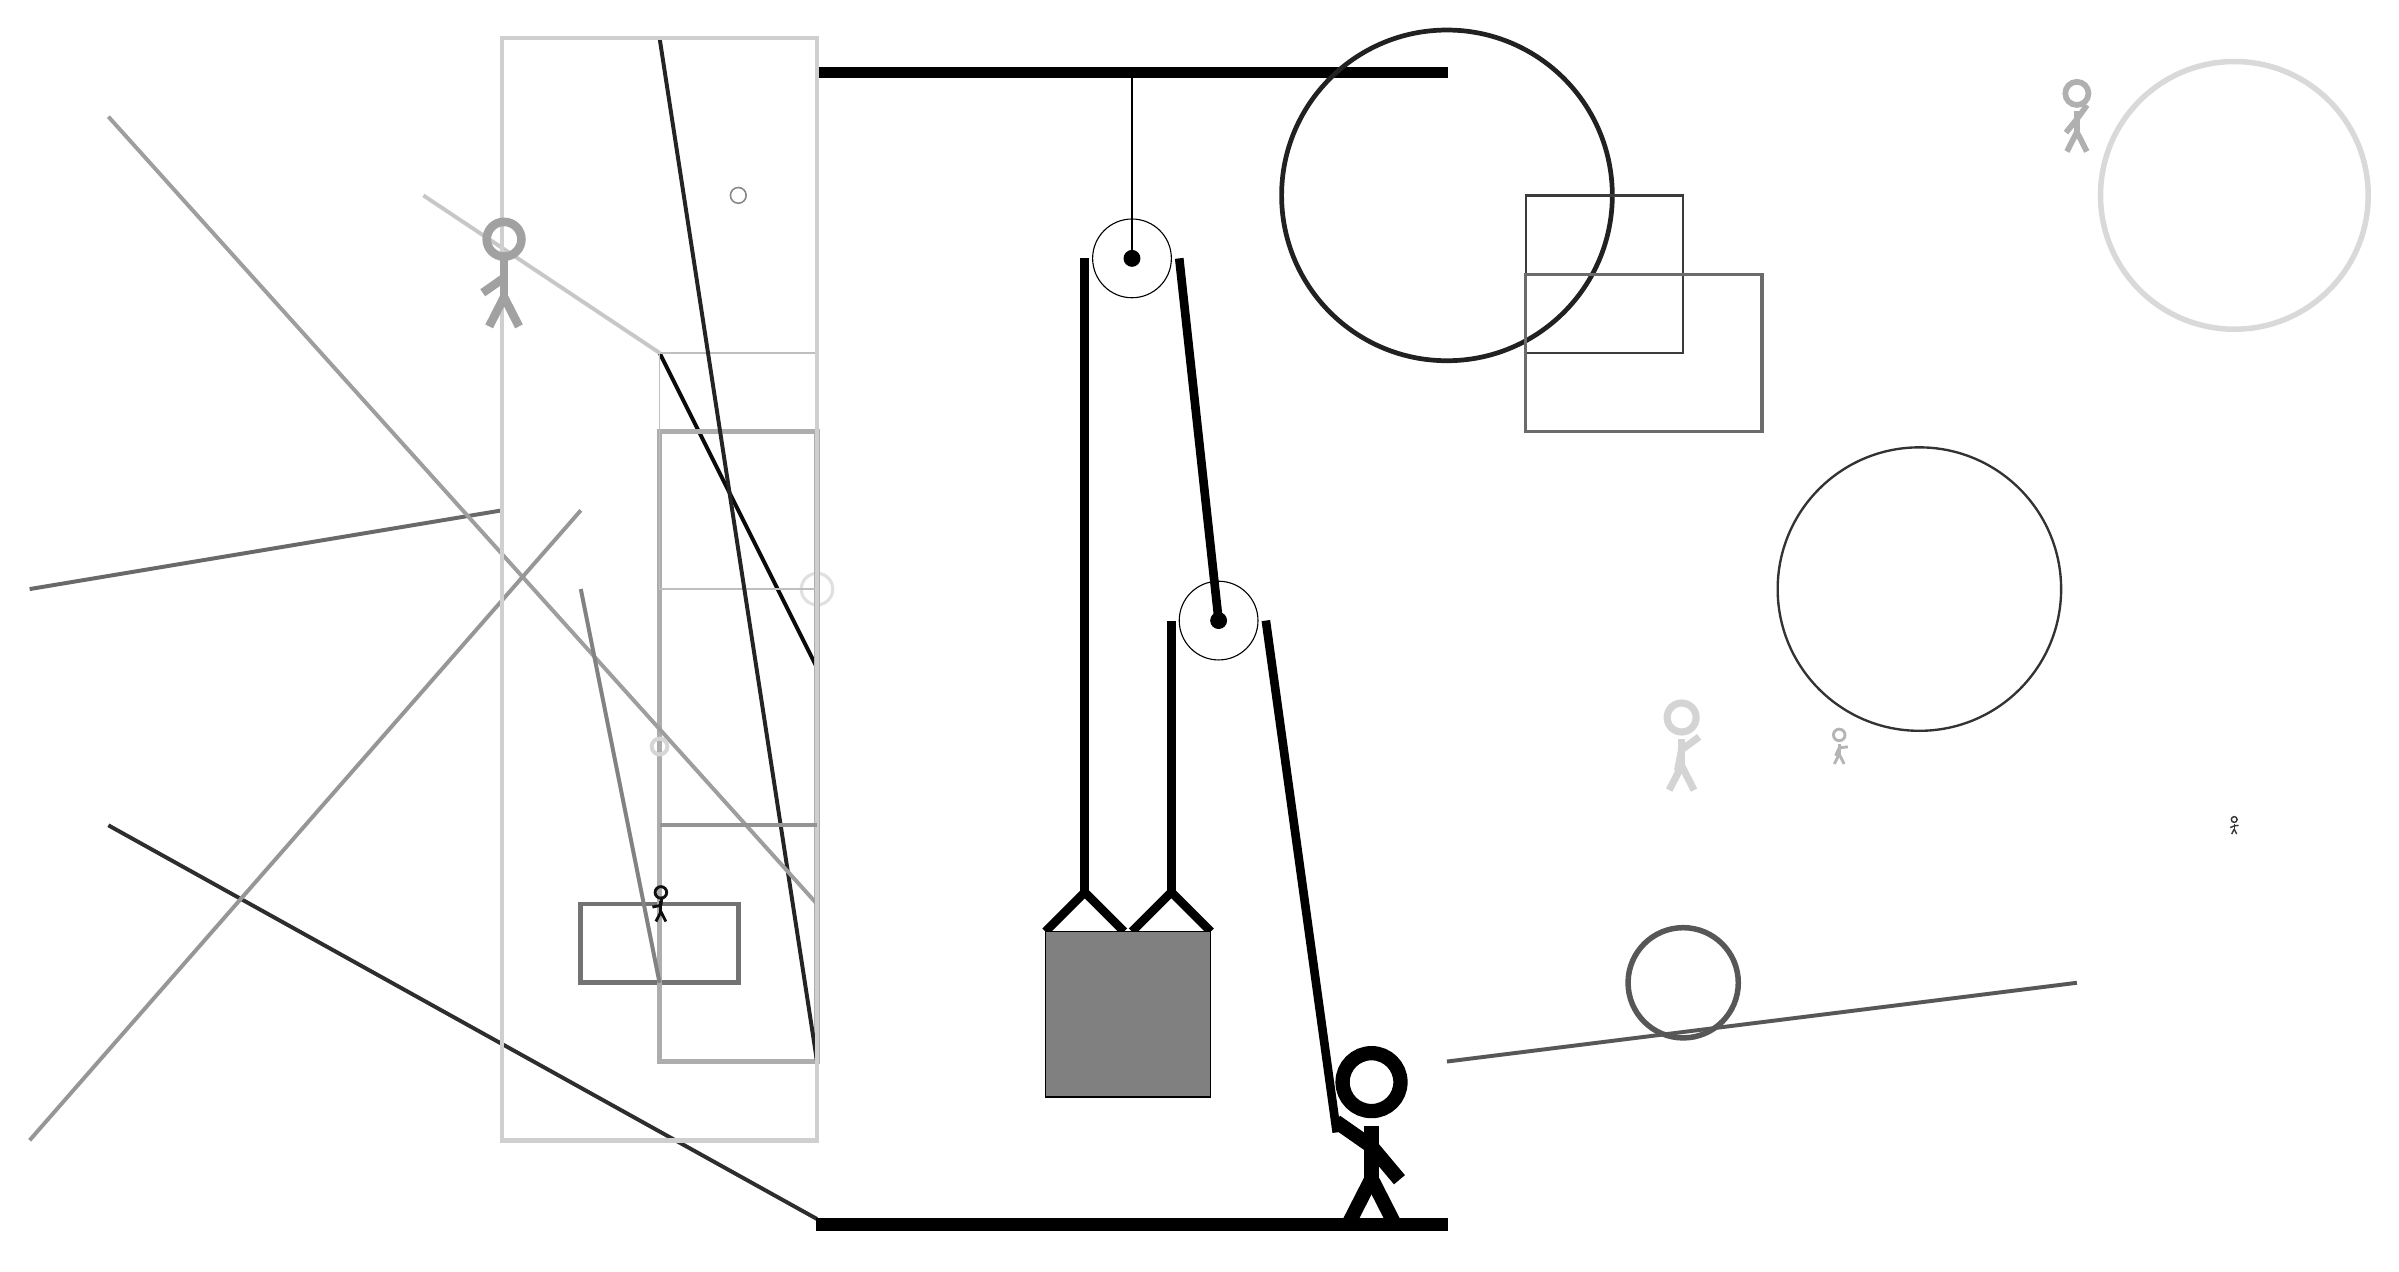
\begin{tikzpicture}
			%%%%% START %%%%%
			
			\draw[fill=black] (-2, 11.5) rectangle (6, 11.625);
			
			\draw[line width=0.6mm, color=black!55] (-3, 1) rectangle (-5, 0);
			
			\draw[line width=0.5mm, color=black!96](-4, 8) -- (-2, 4);
			\draw [line width=0.7mm, color=black!66](9, 0) circle (0.7);
			\node[line width=0.7mm, color=black!29] at (11, 3) {\Strichmaxerl[2][65][6]};
			
			\draw [line width=0.4mm, color=black!12](-2, 5) circle (0.2);
			\draw[line width=0.5mm, color=black!82](-2, -3) -- (-11, 2);
			\draw[line width=0.7mm, color=black!32] (-2, 7) rectangle (-4, -1);
			
			\draw [line width=0.6mm, color=black!87](6, 10) circle (2.1);
			\draw[line width=0.3mm, color=black!77] (7, 8) rectangle (9, 10);
			\draw[line width=0.2mm, color=black!25] (-4, 5) rectangle (-2, 8);
			\draw[line width=0.5mm, color=black!59](-6, 6) -- (-12, 5);
			\draw[line width=0.5mm, color=black!22](-7, 10) -- (-4, 8);
			\draw[line width=0.4mm, color=black!58] (7, 9) rectangle (10, 7);
			
			\draw [line width=0.7mm, color=black!15](16, 10) circle (1.7);
			\draw[line width=0.5mm, color=black!86](-4, 12) -- (-2, -1);
			\draw[line width=0.5mm, color=black!38](-2, 1) -- (-11, 11);
			
			\draw[line width=0.5mm, color=black!66](6, -1) -- (14, 0);
			
			\node[line width=0.7mm, color=black!31] at (14, 11) {\Strichmaxerl[4][51][54]};
			\draw[line width=0.5mm, color=black!41](-5, 6) -- (-12, -2);
			
			\draw [line width=0.5mm, color=black!64](-12, 8) circle (0.0);
			\draw[line width=0.6mm, color=black!19] (-2, -2) rectangle (-6, 12);
			
			\draw[line width=0.5mm, color=black!42](-2, 2) -- (-4, 2);
			\draw [line width=0.3mm, color=black!80](12, 5) circle (1.8);
			\draw[line width=0.5mm, color=black!49](-4, 0) -- (-5, 5);
			\draw [line width=0.2mm, color=black!47](-3, 10) circle (0.1);
			\node[line width=0.3mm, color=black!37] at (-6, 9) {\Strichmaxerl[6][35][90]};
			\node[line width=0.7mm, color=black!79] at (16, 2) {\Strichmaxerl[1][22][8]};
			\node[line width=0.5mm, color=black!94] at (-4, 1) {\Strichmaxerl[2][12][83]};
			
			\node[line width=0.2mm, color=black!17] at (9, 3) {\Strichmaxerl[5][79][36]};
			\draw [line width=0.5mm, color=black!16](-4, 3) circle (0.1);
			
			\draw (2, 9.2) circle (0.5);
			\draw[fill=black] (2, 9.2) circle (0.1);
			\draw[thick] (2, 9.2) -- (2, 11.5);
			
			\draw (3.1, 4.6) circle (0.5);
			\draw[fill=black] (3.1, 4.6) circle (0.1);
			
			\draw[line width = 1.1mm]  (0.9, 0.65) -- (1.4, 1.15) -- (1.9, 0.65);
			\draw[line width = 1.1mm]  (2.0, 0.65) -- (2.5, 1.15) -- (3.0, 0.65);
			\draw[fill=black!50] (0.9, 0.65) rectangle (3.0, -1.45);
			
			\draw[line width = 1.1mm] (1.4, 9.2) -- (1.4, 1.15);
			\centerarc[line width = 1.1mm](2, 9.2)(0:180:0.6);
			\draw[line width = 1.1mm] (2.6, 9.2) -- (3.1, 4.6);
			\draw[line width = 1.1mm] (2.5, 4.6) -- (2.5, 1.15);
			\centerarc[line width = 1.1mm](3.1, 4.6)(0:180:0.6);
			\draw[line width = 1.1mm] (3.7, 4.6) -- (4.6, -1.9);
			
			\node at (5, -2) {\Strichmaxerl[10][-35][-50]};
			
			\draw[fill=black] (-2, -3) rectangle (6, -3.15);
			
			%%%%% END %%%%%
		\end{tikzpicture}
	\end{figure}	
\end{document}